%% Anonymous NSysS 2026 full-paper submission (ACM sigconf, 6--8 pages including references).
\documentclass[sigconf,anonymous]{acmart}

%% Ensure the standard ACM Type 1 font maps are loaded in minimal TeX installations.
\ifpdf
  \pdfmapfile{+libertine.map}
  \pdfmapfile{+zi4.map}
  \pdfmapfile{+newtx.map}
\fi

\usepackage{booktabs}
\usepackage{tikz}
\usetikzlibrary{arrows.meta,positioning,calc}
%% Some minimal TeX installations expose legacy non-scalable math metrics; protrusion remains on.
\microtypesetup{expansion=false}
\emergencystretch=1em

\definecolor{ink}{HTML}{263238}
\definecolor{blue}{HTML}{296C92}
\definecolor{teal}{HTML}{328374}
\definecolor{amber}{HTML}{B97829}

\settopmatter{printacmref=true}
\renewcommand\footnotetextcopyrightpermission[1]{}
\setcopyright{none}
\pagestyle{plain}
\setlength{\textfloatsep}{7pt plus 2pt minus 2pt}
\setlength{\floatsep}{7pt plus 2pt minus 2pt}
\setlength{\intextsep}{7pt plus 2pt minus 2pt}

\acmConference[NSysS 2026]{13th International Conference on Next-generation Computing,
Communication, Systems and Security}{December 17--19, 2026}{Cox's Bazar, Bangladesh}
\acmYear{2026}
\copyrightyear{2026}

\begin{document}

\title{Partition-Tolerant Federation Across Simulated ISP Islands}
\author{Anonymous Author(s)}

\begin{abstract}
National disconnection does not necessarily remove all domestic IP reachability: access networks may
remain as isolated ``islands'' even when international routes disappear. We investigate whether a
signed, server-federated forum can keep accepting and carrying public posts across such residual
paths. The prototype admits byte-canonical protobuf envelopes through a 19-stage validation pipeline,
returns signed transparency receipts, initiates synchronization from either side, and permits an
explicitly trusted dual-homed node to relay between otherwise disjoint islands. In a four-node
container deployment, after removing every inter-island route, certificate, community, and post
objects crossed a bridge in 0.5, 1.2, and 2.1 seconds. After repairing serial head-of-line blocking,
the post case fell from 407.6 seconds to 2.1 seconds. In a separate eight-node in-process chain,
200/200 envelopes reached hop 7 (median 4.125 seconds; p99 6.115 seconds). TypeScript, Rust, and Python
implementations agreed on all 16 canonical vectors. A 3,000-request malformed-envelope run sustained
730 requests/s, but 90\% of requests were rate-limited; the defensible result is zero invalid-object
writes, not denial-of-service resistance. Against 80 measured ActivityPub activities, the proposed
encoding used 4.4--6.9$\times$ fewer bytes than gzipped JSON-LD (19.5--25.9$\times$ fewer than raw
JSON-LD, with caveats). These controlled, single-host results establish a reproducible mechanism for
partition-tolerant federation under surviving domestic IP paths; they do not establish operation in
a total communications blackout or resistance to a coercive network operator.
\end{abstract}

\begin{CCSXML}
<ccs2012>
 <concept><concept_id>10003033.10003099</concept_id>
 <concept_desc>Networks~Network reliability</concept_desc><concept_significance>500</concept_significance></concept>
 <concept><concept_id>10002978.10002997</concept_id>
 <concept_desc>Security and privacy~Distributed systems security</concept_desc><concept_significance>300</concept_significance></concept>
 <concept><concept_id>10002951.10003227.10003351</concept_id>
 <concept_desc>Information systems~Social networks</concept_desc><concept_significance>300</concept_significance></concept>
</ccs2012>
\end{CCSXML}
\ccsdesc[500]{Networks~Network reliability}
\ccsdesc[300]{Security and privacy~Distributed systems security}
\ccsdesc[300]{Information systems~Social networks}

\keywords{network partitions, federated systems, signed objects, transparency logs,
canonical encoding, internet shutdowns}

\maketitle

\section{Introduction}

Shutdown measurements increasingly show a spectrum rather than a binary state: throttling, protocol
interference, destination blocking, and loss of international routes can leave unequal fragments of
connectivity~\cite{ooni2025bangladesh,bischof2023shutdowns}. Baltra et al. call such mutually reachable
fragments \emph{connectivity islands}~\cite{baltra2024connectivity}. This paper asks a deliberately
narrow question: if some domestic IP routes survive, can independently operated forum servers keep
accepting authenticated objects and synchronize them across the remaining graph, including through
a locally trusted relay?

Existing circumvention and blackout systems answer adjacent questions. Proxies and refraction
networking reconnect users to infrastructure outside the filtered region~\cite{wustrow2011telex,
fifield2015fronting,bocovich2024snowflake}. Device-to-device systems disseminate messages without IP
infrastructure~\cite{kamali2025anix,lerner2016rangzen,pradeep2022moby,hossmann2011twimight}. Federated
social protocols assume routable server addresses, while signed-log systems provide integrity without
an operator-oriented admission and receipt workflow~\cite{activitypub,matrixspec,atproto,nostr,
tarr2019ssb}. The unfilled design point is therefore neither global circumvention nor infrastructure-
free delay-tolerant networking. It is \emph{server federation inside partial reachability}, with
verifiable acceptance at each operator boundary.

We present and evaluate a working implementation with four contributions:

\begin{itemize}
  \item a single byte-preserving admission path for local and federated signed objects, with no
        persistent writes in validation stages 1--12;
  \item caller-initiated delivery, streaming, and backfill, allowing a server that cannot accept
        inbound connections to participate by dialing a reachable peer;
  \item policy-constrained bridging by a normal validating server that is explicitly trusted by each
        side and cannot relay an object back over its incoming uplink; and
  \item reproducible evidence from canonical vectors, unit and integration suites, a route-cut
        container experiment, an eight-node chain, and a measured encoding comparison.
\end{itemize}

Our claim is correspondingly limited. The system is \emph{partition tolerant under surviving IP
paths}. It cannot manufacture a route through a physical or radio blackout, hide traffic from deep
packet inspection, or prevent an operator from refusing valid posts.

\section{Background and Research Gap}
\label{sec:background}

\subsection{Existing solution families}

\textbf{Circumvention} systems conceal or redirect a user's connection to an external service.
Telex places anti-censorship logic in cooperating ISP routers~\cite{wustrow2011telex}; domain
fronting and Snowflake exploit alternative rendezvous or proxy surfaces~\cite{fifield2015fronting,
bocovich2024snowflake}. These are valuable when an external path exists, but do not make domestic
servers converge after that path is removed.

\textbf{Blackout messaging} removes the server assumption. Twimight stores and forwards tweets over
opportunistic Bluetooth contacts~\cite{hossmann2011twimight}; Rangzen and Anix combine encounters with
social trust or endorsement~\cite{lerner2016rangzen,kamali2025anix}; Moby targets anonymous messaging
under network blackouts~\cite{pradeep2022moby}. Dolphin instead tunnels through cellular voice at low
bit rate~\cite{sharma2023dolphin}. These systems trade latency, energy, or bandwidth for independence
from domestic IP infrastructure. They do not define a federated public-forum boundary between
operators that still run reachable servers.

\textbf{Federation and signed replication} provide reusable pieces. ActivityPub defines inbox-based
social federation~\cite{activitypub}; Matrix and AT Protocol provide state or repository federation
~\cite{matrixspec,atproto}; Nostr and Secure Scuttlebutt sign replicated content~\cite{nostr,
tarr2019ssb}. FETHR explored decentralized micropublishing at Internet scale~\cite{sandler2009fethr},
while Publius replicated static censorship-resistant documents~\cite{waldman2000publius}. These
systems generally presume routable destinations, or lack the combination of raw-byte admission,
operator receipts, and an explicit two-island relay policy studied here.

\textbf{Accountability} is not availability. Certificate Transparency (CT) makes an append-only log
auditable with signed tree heads and consistency proofs~\cite{rfc6962,rfc9162}; PeerReview and CoSi
show stronger paths to distributed accountability~\cite{haeberlen2007peerreview,syta2016cosi}.
Borrowing CT-style receipts can prove that a server acknowledged an object. It cannot prove that the
server admitted every valid object, forwarded promptly, or resisted coercion.

\subsection{Gap and design objective}

Prior work separates into three substrates: globally routed circumvention, infrastructure-free
encounter networks, and normally routed federation. Hasan identifies the wider challenge of scaling
blackout circumvention while preserving operator safety~\cite{hasan2013dissent}; Baltra et al. provide
the vocabulary for reasoning about partial reachability~\cite{baltra2024connectivity}. We target the
gap between them: IP works \emph{within} or \emph{between some} islands, servers remain online, but
DNS, inbound reachability, or international routing may be unreliable. The objective is to accept an
authored object once, preserve its signed bytes, and make every reachable replica eventually process
the same object under the same rules.

\section{System Design}
\label{sec:design}

\subsection{Object and admission model}

An author creates a protobuf envelope containing a domain tag, object type, payload, public key,
nonce, and expiry. Its identifier is the SHA-256 digest of the specified canonical bytes, and an
Ed25519 signature covers those bytes~\cite{bernstein2012ed25519}. Protobuf does not promise canonical
serialization~\cite{protobufnotcanonical}; the profile therefore fixes field order, rejects unknown
fields, uses minimal varints, and requires decode--re-encode byte equality. The receiver never
``repairs'' attacker-controlled bytes before signature verification.

Local and federated objects enter the same 19-stage pipeline. Stages 1--12 enforce raw size, parse
and canonicality, domain separation, identifiers, signature, expiry, nonce/replay, and semantic
authorization without persistent writes. Later stages apply origin admission or receiver-side peer
quotas, commit the exact raw envelope and derived indexes transactionally, append its hash to a Merkle
log, and enqueue fan-out only after commit. Exact retries are idempotent. Local admission may require
a priced proof; federated reception is quota-bounded because a malicious origin can omit its own
price. We therefore do not claim that origin pricing protects other operators.

On acceptance, the server returns a signed receipt containing the object identifier, leaf position,
signed tree head, and inclusion proof. A client can bind acknowledgment to the submitted bytes.
Receipts make accepted-history equivocation detectable when peers compare sufficient evidence, but
they do not prevent refusal or selective delay.

\subsection{Partition-aware federation}

Three caller-initiated RPCs cover the synchronization cases: \textsc{Deliver} sends a batch,
\textsc{StreamActivities} resumes from a durable cursor, and \textsc{Backfill} retrieves missing
objects. Outbox queues are grouped by source uplink, destination peer, and traffic plane, then drained
concurrently. Each attempt has a scheduler deadline, exponential backoff, and an idempotency key.
The underlying library call is not forcibly cancelled at the deadline, a limitation discussed in
Section~\ref{sec:limits}. Source-address binding and a resolver keyed by source and destination allow
one process to select among simulated ISP uplinks.

Figure~\ref{fig:topology} shows the deployed topology. $R_0$ and $R_1$ share island A; $R_2$ and
$R_3$ share island B. $R_1$ is dual-homed. After the inter-island route is cut, ordinary nodes cannot
dial across islands. Each side explicitly lists $R_1$ as a trusted bridge. The bridge is not a packet
forwarder: it verifies and stores each envelope as a normal server, applies a token bucket per uplink
pair and object class, and never emits an object over the uplink on which it arrived. Bulk backfill
receives half the interactive rate. These rules bound relay volume and loops, but do not make the
bridge covert or safe from coercion.

\begin{figure}[t]
\centering
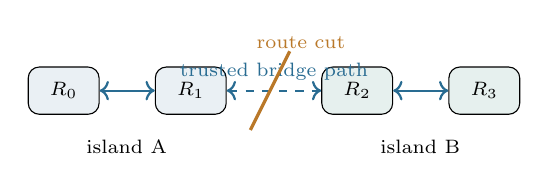
\begin{tikzpicture}[
  node distance=5mm and 7mm,
  n/.style={draw,rounded corners,minimum width=9mm,minimum height=6mm,font=\scriptsize},
  lab/.style={font=\scriptsize},
  arr/.style={-{Latex[length=1.5mm]},thick,blue}]
\node[n,fill=blue!10] (r0) {$R_0$};
\node[n,fill=blue!10,right=of r0] (r1) {$R_1$};
\node[n,fill=teal!12,right=12mm of r1] (r2) {$R_2$};
\node[n,fill=teal!12,right=of r2] (r3) {$R_3$};
\draw[arr,<->] (r0)--(r1);
\draw[arr,<->] (r2)--(r3);
\draw[arr,dashed,<->] (r1)--node[above,lab]{trusted bridge path}(r2);
\node[lab,below=2mm of r0,xshift=8mm] {island A};
\node[lab,below=2mm of r2,xshift=8mm] {island B};
\draw[amber,very thick] ($(r1.east)+(3mm,-5mm)$)--($(r1.east)+(8mm,5mm)$);
\node[lab,amber,above=1mm of r1,xshift=14mm] {route cut};
\end{tikzpicture}
\Description{Four servers arranged as two two-node islands. A dual-homed trusted bridge stores and
relays objects across the otherwise cut route.}
\caption{Four-node virtual topology. The dashed path is application-level storage and relay, not
transparent IP forwarding. All containers run on one physical host.}
\label{fig:topology}
\end{figure}

Peers gossip signed tree heads (STHs). Same-size/different-root and a smaller new head at a later
trusted time are strong conflicts. An older timestamp is ignored as stale. A larger tree is recorded
as \emph{pending} rather than declared consistent: growth requires a CT consistency proof. Thus the
current mechanism provides stale-head suppression and some conflict detection, not complete fork
detection for growing trees.

\subsection{Replication and recovery invariants}

The implementation enforces four invariants at adapter boundaries. First, federation transports an
opaque byte string into ingress. A generated RPC decoder must not deserialize and then serialize an
envelope, because doing so could silently normalize a non-canonical attack into an accepted object.
Second, peer trust changes volume and priority policy, never validity: even an explicitly configured
bridge must pass signature, identifier, expiry, replay, and authorization checks. Third,
deduplication is a database uniqueness constraint on content identifier and direction rather than a
read-before-write check. This matters when a live stream and a backfill concurrently deliver the
same object. Fourth, fan-out excludes the origin peer. Content deduplication would eventually stop a
loop, but origin exclusion avoids paying a redundant round trip for every accepted object.

Identifiers for projected entities are derived only from signed envelope fields. This rule was added
after an early projector used the receiving node's key when constructing a community identifier. A
single-node test could not reveal the error; two nodes produced permanently different projections
from the same signed object. The corrected implementation asks whether any node with only the signed
bytes will derive the same identifier. Dependency objects are admitted before their dependents, and
missing dependencies remain retryable rather than being partially projected.

Durable cursors make recovery independent of a continuously open connection. A caller presents its
last accepted cursor, the peer streams later activities, and exact retries are absorbed by the unique
index. Backfill uses the same path for an explicit missing range. Consequently, a node advertising no
inbound endpoint can still send its own outbox and retrieve the peer's history over connections that
it initiates. This supports asymmetric reachability such as carrier-grade NAT, but requires at least
one side to know a reachable peer address. It is not peer discovery.

Strict canonicality also constrains evolution. An old implementation rejects unknown fields instead
of forwarding data it cannot authenticate under its own profile. Compatible schema changes therefore
need a versioned domain or envelope profile and cross-language vectors for both versions. We accept
this upgrade cost to keep the signed byte string unambiguous.

\section{Methodology}
\label{sec:method}

We evaluate five questions: (RQ1) do independent encoders agree; (RQ2) do objects cross an enforced
route cut; (RQ3) does propagation remain complete over multiple hops; (RQ4) do malformed requests
become storage writes; and (RQ5) what is the wire-size difference from a deployed federation format?

\textbf{Correctness suites.} A shared corpus contains 16 positive and adversarial byte vectors. It is
executed independently by TypeScript, Rust, and Python implementations. The backend suite exercises
the ingress, outbox, federation, and ISP abstractions. At revision time, 85 focused tests passed (29
ingress, 3 outbox, 31 federation, and 22 ISP tests), in addition to the vector gate. These are
in-process checks and are not counted as deployment measurements.

\textbf{Four-node route-cut deployment.} Four application containers, four databases, and four
caches are attached to three private Docker networks. The gate records source/destination reachability
from kernel TCP state, removes the only ordinary inter-island path, proves that direct island-A to
island-B probes fail, submits a dependency chain (issuer certificate, community, post), and polls the
destination for each exact content identifier. The bridge has fixed addresses on both island
networks. Reported times are end-to-end wall-clock observations from this gate, including application
polling. Because all containers share one physical host, the experiment validates routing and
software state transitions, not geographic latency, independent failure domains, or ISP behavior.

\textbf{Eight-node chain.} An in-process harness links eight servers in a line. It injects 200 valid
envelopes at hop 0, waits for all to reach hop 7, and records per-object completion latency. This
isolates the federation scheduler but omits container networking and durable external services.

\textbf{Invalid-envelope run.} A client sends 3,000 over-sized or non-canonical requests at
concurrency 16 to one node. We measure completion rate, rejection classes, signature-verification
entries, and persistent object count. The node's normal limiter remains enabled; hence throughput is
descriptive of the configured gate, not a saturation benchmark.

\textbf{Encoding comparison.} We collected 80 activities emitted by two stock ActivityPub
implementations, retained the delivered JSON-LD contexts, and compared delivered and gzip-compressed
bytes with equivalent signed protobuf envelopes. We subtract authored text to estimate overhead but
do not include HTTP framing, ActivityPub HTTP signatures, TLS records, follower fan-out, or
compression dictionaries. The comparison addresses representation size, not total protocol cost.

\textbf{Reproducibility boundary.} The artifact contains the compose topology, route gate, canonical
fixtures, and deterministic test entry points; generated bindings are checked for drift. The focused
suites and vector gate were rerun for this revision. Route-cut numbers come from the deployment
gate's preserved output. Random seeds, host load, repeated-run distributions, and confidence
intervals were not preserved for those observations; they should be added before drawing
performance-generalization claims.

\section{Results}
\label{sec:results}

\subsection{Correctness and convergence}

\textbf{RQ1.} All three independent implementations produced identical output for 16/16 canonical
vectors and rejected every negative vector as specified. This is evidence that the wire profile is
implementable across languages; sixteen fixtures are not a proof that all protobuf edge cases are
covered.

The focused suites also exercise failures that the happy path can hide: corrupted signatures,
non-canonical encodings, identifier disagreement, replay, missing authorization dependencies,
concurrent duplicate delivery, a receipt under the wrong key, an inclusion proof for different
content, stale STHs, same-size/different-root conflicts, and shrinking trees. Growing STHs are expected
to enter the pending state, reflecting the missing consistency proof rather than being reported as
safe. The 85-test count is useful regression evidence, but it combines unit and in-process integration
tests and is not an independent security audit.

\textbf{RQ2.} The deployment gate completed 19/19 assertions. With direct inter-island reachability
removed, the destination observed the certificate after 0.5 seconds, the dependent community after
1.2 seconds, and the post after 2.1 seconds. A prior implementation drained destinations serially and
allowed one blackholed peer to block every following peer; the same post path then took 407.6 seconds.
Grouping queues per peer/uplink and draining them concurrently reduced this observation by 99.5\%.
The result explains the improvement: it removes unrelated head-of-line wait, rather than accelerating
cryptography or transport.

\textbf{RQ3.} All 200 envelopes reached hop 7. End-to-end median was 4.125 seconds and p99 was 6.115
seconds. Figure~\ref{fig:chain} shows the monotonic hop cost. The modest p99--median gap is consistent
with bounded parallel draining in this low-contention harness; the experiment does not model WAN
jitter or adversarial valid traffic.

\begin{figure}[t]
\centering
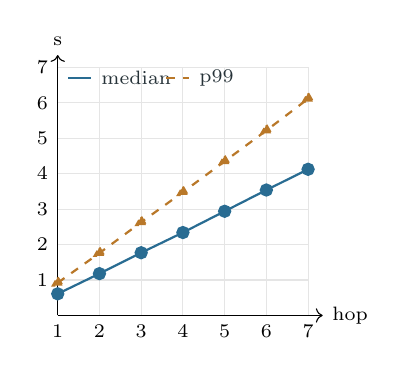
\begin{tikzpicture}[x=.53cm,y=.45cm,font=\scriptsize]
\draw[gray!20,step=1] (1,0) grid (7,7);
\draw[->] (1,0)--(7.35,0) node[right]{hop};
\draw[->] (1,0)--(1,7.35) node[above]{s};
\foreach \x in {1,...,7} \node[below] at (\x,0) {\x};
\foreach \y in {1,...,7} \node[left] at (1,\y) {\y};
\draw[blue,thick] plot[mark=*] coordinates
  {(1,.61)(2,1.18)(3,1.77)(4,2.34)(5,2.94)(6,3.54)(7,4.125)};
\draw[amber,thick,dashed] plot[mark=triangle*] coordinates
  {(1,.92)(2,1.76)(3,2.63)(4,3.48)(5,4.35)(6,5.22)(7,6.115)};
\draw[blue,thick] (1.25,6.7)--(1.8,6.7) node[right,ink]{median};
\draw[amber,thick,dashed] (3.6,6.7)--(4.15,6.7) node[right,ink]{p99};
\end{tikzpicture}
\Description{A line plot in which median and p99 completion time increase approximately linearly
from hop one to hop seven. At hop seven the values are 4.125 and 6.115 seconds.}
\caption{Eight-node in-process chain, 200/200 envelopes delivered. Intermediate-hop values are
recorded observations; hop 7 is the reported end-to-end result.}
\label{fig:chain}
\end{figure}

\subsection{Admission and representation cost}

\textbf{RQ4.} The invalid run completed at 730 requests/s and produced zero object, index, log, or
outbox writes. However, 2,700/3,000 requests (90\%) were stopped by rate limiting; only about 9\%
entered signature verification. The sound conclusion is that the tested malformed traffic did not
amplify into invalid-envelope storage writes. It is not evidence of denial-of-service resistance:
valid signed floods, distributed sources, parsing allocation, and database contention remain open.

\textbf{RQ5.} Table~\ref{tab:size} leads with the compression-aware comparison. For matched post,
follow, and delete objects, gzipped ActivityPub was 4.4--6.9$\times$ larger. Raw JSON-LD overhead was
19.5--25.9$\times$ larger, but that ratio advantages a binary format by ignoring routine HTTP
compression. The gzip result is the more operationally relevant observation.

\begin{table}[t]
\caption{Representation bytes over 80 measured ActivityPub activities. Ratios compare ActivityPub
with the proposed envelope after subtracting authored text.}
\label{tab:size}
\centering
\small
\begin{tabular}{lrrr}
\toprule
 & Post & Follow & Delete \\
\midrule
Proposed envelope & 206 & 142 & 250 \\
ActivityPub, gzip & 1,074 & 786 & 1,400 \\
Gzip ratio & 5.2$\times$ & 5.5$\times$ & 5.6$\times$ \\
Observed range & \multicolumn{3}{c}{4.4--6.9$\times$} \\
ActivityPub, raw & 4,216 & 2,786 & 6,909 \\
Raw overhead ratio & 19.5$\times$ & 19.5$\times$ & 25.9$\times$ \\
\bottomrule
\end{tabular}
\end{table}

\subsection{Qualitative and quantitative comparison}

Table~\ref{tab:related} places the results beside systems with different substrates and threat
models. The values are intentionally not normalized: ``delivery'' means server-to-server convergence
here, encounters in Anix/Rangzen/Twimight, modeled visibility in GhostPost, and a trace-driven flood
in Moby. Sample size and evaluation method are therefore shown in the same cell.

\begin{table*}[t]
\caption{Comparison with representative prior systems. Values retain each paper's own denominator
and workload; they are context, not a cross-system ranking. ``IP federation'' means an evaluated
server-to-server path under partial reachability.}
\label{tab:related}
\centering
\scriptsize
\setlength{\tabcolsep}{3.1pt}
\begin{tabular}{p{1.55cm}p{2.05cm}p{1.55cm}p{3.35cm}p{2.1cm}p{2.55cm}}
\toprule
System & Substrate & Public/authored integrity & Reported quantitative evidence & Partial-IP federation & Principal distinction \\
\midrule
This work & Surviving IP; trusted dual-uplink relay & Yes; Ed25519 envelope + receipt & 4-node route cut: 0.5/1.2/2.1 s; 8-node chain: 200/200, hop-7 p50 4.125 s, p99 6.115 s & Yes, four-node virtual topology & Operator-oriented signed admission and resumption \\
Anix~\cite{kamali2025anix} & Bluetooth/Wi-Fi Direct & Public anonymity + endorsement & 600 simulated users; $>$90\% dissemination in about 23 h; discovery 1.8 s, exchange 11.58 s & No & Infrastructure-free opportunistic spread \\
Rangzen~\cite{lerner2016rangzen} & Phone encounters & Anonymous social-trust dissemination & 400-node main simulation, 40-run means; $>$80\% in 24--48 h; encounter 6.61 s & No & Friend-to-friend trust under blackout \\
Moby~\cite{pradeep2022moby} & Mobile opportunistic network & Private anonymous messaging & 268,596-user trace basis; highlighted flood 13.96\% vs. 1.15\% epidemic delivery & No & Stronger privacy/forward secrecy objective \\
Twimight~\cite{hossmann2011twimight} & Bluetooth store-and-forward & Authenticated disaster tweets & 5 users, 915 tweets; almost all delivered in about 2 h; 41--68 h battery & No & Early deployed disruption-mode client \\
Dolphin~\cite{sharma2023dolphin} & Cellular voice to gateway & Encrypted low-rate tunnel & 64 bit/s, $<$2\% error; secure setup about 60 s; 500-character email about 160 s, 30 trials & No & Works without packet data, at low throughput \\
GhostPost~\cite{douglas2016ghostpost} & Browser caches/social graph & Restores already observed posts & 1M simulated users; about 1.5\% adoption preserves a majority of modeled 30-min views & No & Restoration after platform deletion \\
Secure Scuttlebutt~\cite{tarr2019ssb} & Peer replication & Signed append-only author logs & Operational community reported above 10,000; no controlled partition-latency result & No server path evaluated & Closest signed offline log lineage \\
FETHR~\cite{sandler2009fethr} & Routable HTTP/callback & Decentralized micropublishing & 4,917,042-message/472,735-user trace; about 120k items processed by prototype & Normally routed only & Large trace, but no route-cut metric \\
Publius~\cite{waldman2000publius} & Reachable replicated web servers & Threshold-based static publication & Prototype of about 1,500 lines; analytical/functional evaluation & Normally routed only & Static-document availability \\
\bottomrule
\end{tabular}
\end{table*}

The comparison exposes complementarity rather than dominance. Encounter systems operate when IP is
absent but converge over hours and consume scarce handset energy. The proposed server path converges
in seconds in a virtual topology but requires powered, mutually reachable infrastructure. Dolphin can
cross a packet-data shutdown but its 64-bit/s channel is unsuitable for routine federation. Normally
routed federation and static replication scale to larger observed corpora, yet their cited
evaluations do not test the route-cut and dual-homed relay case. Our experiment fills that narrow gap;
it is far smaller than the trace and simulation studies in Table~\ref{tab:related}.

\section{Discussion}
\label{sec:discussion}

\textbf{Why did the bridge result improve?} The 407.6-second failure was a scheduling artifact: one
unreachable destination monopolized a serial drain. Per-peer concurrent queues make progress on a
reachable bridge independent of that destination, producing the 2.1-second result. Deadlines alone
would cap, rather than remove, cross-peer interference; unrestricted concurrency would improve an
idle test yet allow a valid flood to consume memory and sockets. The chosen bounded concurrency is a
middle path, although the uncancelled underlying call still deserves repair.

\textbf{What if we had chosen device-to-device networking?} Bluetooth or Wi-Fi Direct would extend
operation to a total IP blackout and remove the dual-homed-server dependency. Prior results suggest a
different operating regime: encounter-based convergence in hours, discovery overhead, handset
battery cost, and difficult background execution. A hybrid design could carry the same signed
envelope over opportunistic links, but peer discovery, privacy, duplicate suppression, and mobile
energy would become primary research questions. Our seconds-scale server results cannot predict that
hybrid's behavior.

\textbf{What if we had reused ActivityPub JSON-LD?} Interoperability and an existing application
ecosystem would improve. The measured raw representation would be substantially larger, though gzip
narrows the difference to 4.4--6.9$\times$. More importantly, signing ActivityPub across JSON-LD
processing requires an agreed canonicalization and authentication profile. Conversely, selecting a
custom canonical protobuf reduces bytes and makes the verified byte string explicit, but creates a
new interoperability burden and a risk that untested codecs disagree. The 16-vector, three-language
gate reduces rather than eliminates that risk.

\textbf{What if receivers normalized incoming bytes?} Decode--normalize--verify would make benign
codec variation easier to accept and would ease rolling upgrades. It would also make the receiver,
rather than the author, choose the signed representation. Two libraries could accept different byte
strings for the same logical message, complicating content identifiers, replay detection, and receipt
evidence. Raw-byte preservation keeps those properties simple, while versioned profiles carry the
compatibility cost. An alternative worth evaluating is a formally specified deterministic protobuf
subset with differential fuzzing substantially larger than the present 16-vector corpus.

\textbf{Global consensus ordering.} A Byzantine consensus group or
witness-cosigned log could strengthen global non-equivocation~\cite{syta2016cosi}. During a partition,
however, quorum placement would decide which island can write, undermining local availability. The
current per-operator logs preserve independent admission and later evidence exchange. The price is
weaker accountability: a receipt proves acknowledged inclusion only, and growing STHs remain pending
until consistency proofs are implemented.

\textbf{What if bridges were automatic?} Discovering and accepting any dual-homed node would improve
reachability but turn it into an attractive Sybil, eclipse, and traffic-amplification surface.
Explicit bilateral trust limits that surface and makes operator responsibility visible, at the cost
of manual configuration and a conspicuous chokepoint. Multiple disjoint bridges and signed policy
distribution would reduce single-relay dependence, but were not evaluated.

\textbf{Interpreting the measured boundaries.} The multi-hop curve grows roughly linearly because
each hop waits for local validation, storage, and the next bounded drain. That behavior is appropriate
for a short server path and less attractive for a long overlay. The zero-write invalid run follows
from placing cheap byte and canonical checks before state changes, but the 90\% limiter share means it
mostly demonstrates configured admission ordering. Finally, the representation result is largest
against uncompressed JSON-LD and smaller against gzip; compression-aware numbers should guide
deployment expectations.

\section{Limitations, Threats, and Ethics}
\label{sec:limits}

\textbf{External validity.} The strongest limitation is scale and realism. The deployed topology has
four nodes on one physical machine; the chain has eight in-process nodes; there is one measured
route-cut run reported by the gate. Shared CPU, clock, storage, and kernel remove geographic latency
and correlated infrastructure failures. No field shutdown, ISP cooperation, mobile client, human
moderation workload, or multi-day reconnection was studied. The related-work quantities use different
substrates and denominators and must not be read as a leaderboard.

\textbf{Network adversary.} A domestic operator can identify stable endpoints, apply IP or SNI
whitelists, fingerprint gRPC/TLS traffic, perform traffic analysis, coerce a bridge, or isolate nodes
into an eclipse. Source binding does not conceal an endpoint. A total power, radio, and packet outage
leaves no path. The design should therefore be described as partition tolerant, not censorship
resistant. Operational exploration would require endpoint rotation, pluggable transports, bridge
diversity, and explicit risk assessment for local operators.

\textbf{Application adversary.} Signatures authenticate keys, not truth or safety. A malicious author
can submit abuse; a valid-key flood can pass the early cryptographic gate; a malicious origin can skip
its own admission price; and receiver quotas may still permit costly work. Key theft, metadata leakage,
moderation, revocation recovery, storage exhaustion, and coordinated Sybil behavior remain open.
The scheduler deadline does not cancel the underlying RPC. The current STH rule suppresses stale heads
and detects some conflicts, but cannot establish append-only growth without consistency proofs.

\textbf{Accountability boundary.} Operator-signed receipts are evidence of acknowledged acceptance,
not proof of universal availability. A server can refuse to issue a receipt, selectively withhold an
accepted object, show different histories to disconnected peers, or delay until evidence expires.
Independent witnesses, consistency proofs, and eventually PeerReview- or CoSi-like mechanisms could
strengthen detection, but cannot force service under coercion.

\textbf{Ethics.} The experiments used synthetic content and isolated private networks; they did not
interact with production services or real users. A real deployment could expose bridge operators and
users to legal or physical risk. Publication of a protocol should not be mistaken for advice to run a
visible relay in a hostile jurisdiction. Threat modeling, informed consent, data minimization, and
local legal and community review are prerequisites for field work.

\section{Conclusion}

This work demonstrates a narrow but useful point: when domestic IP fragments remain, server
federation need not stop merely because normal inter-island routing does. A byte-canonical signed
object, common validation path, caller-initiated synchronization, and explicitly trusted validating
bridge carried a dependency chain across an enforced virtual route cut, while bounded per-peer
draining removed a severe head-of-line delay. Cross-language vectors and an eight-node chain provide
additional correctness evidence, and the comparison clarifies where this server-based design sits
relative to encounter, voice-channel, and normally routed systems. The evidence is controlled and
small-scale. The next steps are CT consistency proofs, cancellation-aware transport, multi-host and
wide-area experiments, valid-traffic stress tests, multiple independent bridges, and a hybrid
opportunistic transport for periods in which IP disappears entirely.

\balance
\bibliographystyle{ACM-Reference-Format}
\bibliography{references}

\end{document}
